% English version of paper/ja_v2/05_問い1b.md (2026-11-17).
\section{RQ1(b): distillation raised the point estimate of audio UAR in all 12 conditions, and UAR rose only when the pseudo-labels had higher UAR}\label{sec:rq1b}

RQ1(b) asks which classifiers distillation improves and when. In the LOCO setting, the audio classifier had higher UAR than the K-label baseline in all 12 conditions with 5, 10 and 25 labels per emotion (point estimates), and 11 methods that do not use pseudo-labels including other modalities had lower audio UAR than distillation in all 132 comparisons (point estimates). Across the 360 post hoc pseudo-label variants per K (K = 5, 25; pseudo-labels made only of the retrained classifier's own predictions and duplicates of other providers excluded), the UAR of the audio, visual, text and AVT classifiers rose only when the UAR of the pseudo-labels exceeded that of the classifier before retraining.

\subsection{Setting}

\subsubsection{Distillation}\label{sec:distill}
In the LOCO setting we retrain the audio, visual and text classifiers and the AVT classifier. The pseudo-label $q_i$ of each candidate utterance is made in two stages (Fig.~\ref{fig:plflow}). In the first stage, the AVT K-label baseline assigns emotion probabilities to the candidates. In the second stage, the audio, visual and text classifiers are retrained from the anchor on the K labels and these probabilities, and their three probabilities are multiplied per utterance and normalised (the \emph{product}). $q_i$ includes the prediction of the retrained classifier's own modality.

\begin{figure}[t]
\centering
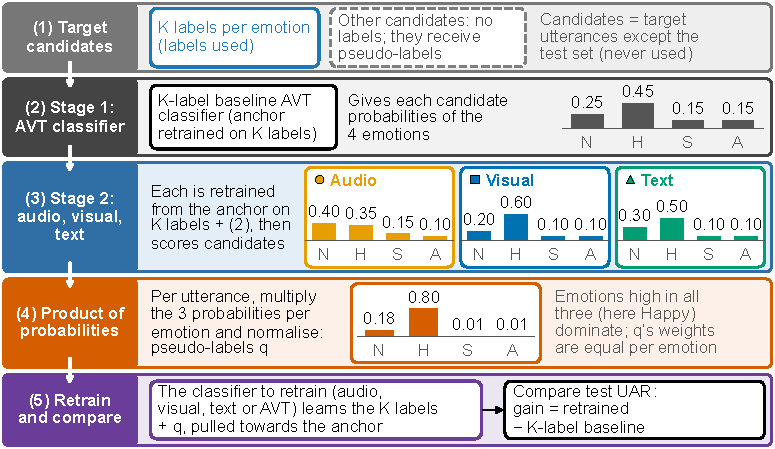
\includegraphics[width=\textwidth]{figures/fig_pl_flow_en.pdf}
\caption{Making and using the pseudo-labels of distillation. The AVT K-label baseline assigns probabilities to the candidate utterances, the audio, visual and text classifiers are retrained on the K labels and these probabilities, their product becomes the pseudo-label, and the classifier is retrained on the K labels and the pseudo-labels and compared on the test UAR. Test utterances are never used before the comparison. The probabilities are illustrative. The proposed fusion of RQ2 replaces the product step}\label{fig:plflow}
\end{figure}

The main loss (form (a)) of the retrained linear classifier is the cross-entropy on the K labels plus the cross-entropy towards the pseudo-labels of the candidates (the pseudo-label probabilities are targets without temperature) plus L2 terms towards the anchor $(W_0,b_0)$:
\begin{equation}
\begin{split}
L(W,b)=\frac{1}{S}\Big[&a\sum_{i\in\mathcal{K}}-\log p(y_i\mid x_i)+\sum_{i\in\mathcal{U}}\sum_k g_{ik}\,(-\log p(k\mid x_i))\\
&+\frac{\|W-W_0\|^2}{2C'}+\frac{\|b-b_0\|^2}{2C_b}\Big],
\end{split}
\end{equation}
with $p(\cdot\mid x)=\mathrm{softmax}(Wx+b)$ and $g_{ik}=(\rho n/4)\,q_{ik}/\sum_{j\in\mathcal{U}}q_{jk}$, where $\mathcal{K}$ is the set of K labelled utterances, $\mathcal{U}$ is the set of all $n$ candidates (including $\mathcal{K}$) and $S$ is the sum of the loss weights. The pseudo-label weights $g_{ik}$ sum to $\rho n/4$ for each emotion $k$. In this paper, \emph{distillation} means retraining with form (a) towards the product. The main loss was fixed as form (a) before the evaluation run. For comparison, five other loss forms that take the pseudo-labels were trained in the same way, and for each target, classifier and K the form with the highest provisional-target UAR was compared with form (a): a temperature loss (form (b)) \cite{hinton2015distilling} with $\tau=2$ from Albanie et al.\ \cite{albanie2018}, pseudo-labels on agreeing utterances only \cite{shi2024audioguided}, mixing with the classifier's own predictions \cite{zhang2021combining}, soft co-training (our variant of the idea of \cite{blum1998}) and co-regularisation \cite{sindhwani2005coreg}; each adapts the loss of the original paper to take the pseudo-labels as targets and is not identical to the original method. $C'$ and $C_b$ are those of the K-label baseline; $\rho\in\{1/16,1/4,1,4\}$, $a\in\{1,4,16\}$ and the exponents of each modality in the product (63 combinations of $\{0,0.5,1,2\}^3$ excluding all zeros) were chosen by the highest mean provisional-target UAR; when several points were within two standard errors of the best, the one closest to the untuned values ($\rho=1$, $a=1$, exponents (1, 1, 1)) was chosen. The values were fixed and recorded in a version-controlled file before the single evaluation run. The authors inspected UARs and differences (without intervals) of the methods during the evaluation run (AFEW, IEMOCAP) and before aggregation; aggregation scripts were fixed beforehand and not changed.

\subsubsection{Comparison methods}
Distillation is compared with 11 methods that do not use pseudo-labels from classifiers including other modalities; they use same-modality unlabelled utterances, labelled source utterances, or mutual imitation between unimodal classifiers. All start from the same anchor and K labels and select hyperparameters by the same procedure.
\begin{itemize}
\item \textbf{Same-modality unlabelled utterances:} self-training \cite{lee2013pseudolabel}, entropy minimisation \cite{grandvalet2004}, IM \cite{liang2020,boudiaf2020}, T3A \cite{iwasawa2021}, label propagation \cite{zhou2004,iscen2019}, and form (a) with the classifier's own K-label-baseline probabilities as pseudo-labels.
\item \textbf{Labelled source utterances:} training on source utterances and the K labels together (S+T), CORAL \cite{sun2016coral}, DANN \cite{ganin2016dann} and MME \cite{saito2019mme}.
\item \textbf{Mutual imitation:} an xMUDA-style method \cite{jaritz2020xmuda} between unimodal classifiers.
\end{itemize}
Because the encoders are frozen, DANN and MME are versions with their loss terms on a linear map and classifier, not the original methods that also train the feature extractor.

\subsubsection{Advantage of the pseudo-labels}\label{sec:margin}
To relate the gain of distillation to how often the pseudo-labels are correct, we compare retraining with different pseudo-label providers. The evaluation run had also retrained each of the four classifiers on predictions of other classifiers instead of the product (untuned $\rho=1$, $a=1$). The providers are K-label baselines (unimodal classifiers of other modalities, classifiers on two concatenated modalities, AVT), the product, the three classifiers that make the product, the AVT anchor and the classifiers of each source corpus. For each variant we measure (Fig.~\ref{fig:margintoy}):
\begin{itemize}
\item the \emph{advantage}: UAR of the provider's decisions $-$ UAR of the classifier before retraining (K-label baseline), on candidates excluding the K labels, using candidate labels that are never used for retraining;
\item the \emph{gain}: UAR of the retrained classifier $-$ UAR of the K-label baseline on test utterances.
\end{itemize}

\begin{figure}[t]
\centering
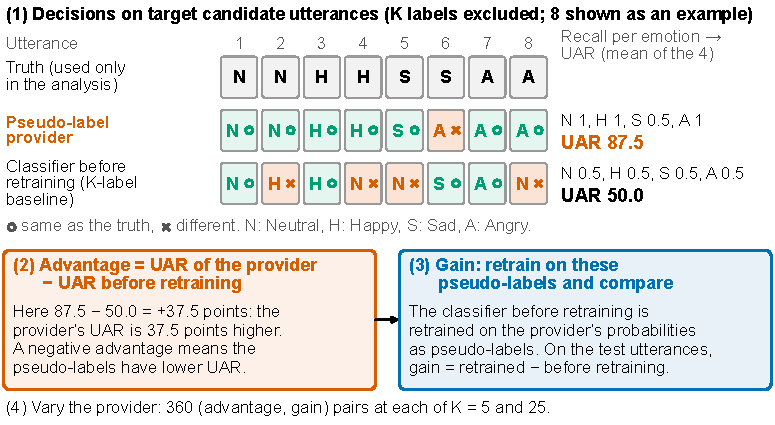
\includegraphics[width=\textwidth]{figures/fig_margin_toy_en.pdf}
\caption{Measuring the advantage and the gain. For candidate utterances, the true labels (used only for this analysis), the decisions of the pseudo-label provider and those of the classifier before retraining give two UARs; the advantage is their difference. The classifier is then retrained on the pseudo-labels and the gain is measured on test utterances. Utterances and decisions are illustrative, not experimental values}\label{fig:margintoy}
\end{figure}

K is 5 and 25, for which the candidate decisions of the K-label baselines were saved. Excluding AVT retrained on its own predictions and duplicates of other providers leaves 360 variants per K. One excluded variant (MOSEI, AVT, K = 25), whose advantage is zero by construction because the provider makes the same predictions as the classifier before retraining, had a gain interval above zero (+0.30 [+0.07, +0.54]). This is a descriptive analysis set up after the computation, without prior predictions; the authors had seen the gains and intervals of some providers before setting it up. Variants share candidates, test utterances and pseudo-label ingredients, so the rank correlations and counts below are not tests.

\subsubsection{How well audio features predict the text classifier's decisions}\label{sec:repro}
As one candidate reason for the audio gains, we examine the explanation that speech carries both voice quality and the spoken words: the product contains the text classifier's decisions, so if audio features can predict those decisions, the audio classifier can learn that part from the pseudo-labels. The cross-modal predictability $D$ is measured as follows: the decisions $J$ of one modality's K-label baseline (e.g., text) are the target; a linear classifier on another modality's features (e.g., audio) predicts $J$ out of sample, and its UAR with $J$ as truth is $R$; the same is done after permuting $J$ within strata of true emotion and speaker cluster (and gender for IEMOCAP and AFEW), giving $R'$; and $D=R-R'$ is the agreement not explained by emotion and speaker. The decision rule was fixed at K = 5 before computing, and AFEW, whose text is a transcript of its own audio, was excluded from the audio--text comparison. We also rebuilt the last-layer WavLM-large features of time-reversed speech of IEMOCAP (improvised), MOSEI and MELD and measured the same $D$ (predictions and rules fixed before computing; the question was set after seeing the non-reversed results). On reversed speech, Whisper large-v3 transcripts agreed with the original words only 0.005--0.012 above chance (0.79--0.80 for the original speech).


\subsection{Results}

\subsubsection{Audio UAR was higher in all 12 conditions in point estimates}\label{sec:rq1b-audio}
Table~\ref{tab:gain} shows the gain of distillation over the K-label baseline. For audio, the gain was positive in all 12 conditions with K = 5, 10 and 25, with intervals above zero for AFEW, MOSEI and MELD at all three K (AFEW +3.32 to +4.15, MOSEI +3.19 to +4.11, MELD +2.71 to +3.12\pt); IEMOCAP gained +1.45 to +2.41\pt\ with intervals including zero. Without labels (K = 0), the audio gain was +2.13 (MOSEI) to +4.86 (AFEW)\pt\ with intervals above zero for all four corpora, and the audio classifier retrained on unlabelled utterances and pseudo-labels alone (K = 0) had higher UAR than the K-label baselines with 5 and 10 labels per emotion in all four corpora (AFEW 53.4 vs 50.1 and 51.1, IEMOCAP 69.2 vs 67.1 and 68.3, MOSEI 36.5 vs 34.9 and 35.1, MELD 45.2 vs 41.5 and 41.8; no intervals computed). Text gained +5.01 to +7.34\pt\ on IEMOCAP at K = 5, 10 and 25 with intervals above zero and had intervals including zero elsewhere; visual intervals were above zero only for MOSEI at K = 10 and 25, and AVT intervals only for MELD at all K and MOSEI at K = 25. Replacing form (a) by the form selected on provisional targets (form (b) in all 16 audio conditions with K = 0, 5, 10, 25) changed audio UAR by $-$0.79 to +0.87\pt, and the selected hyperparameters gave the same classifier as the untuned values in all 16 audio conditions.

\begin{table}[t]
\caption{LOCO setting: gain of distillation over the K-label baseline (UAR points on test utterances) with 95\% intervals without correction. Values average 50 repetitions (5 for K = 0). At K = 0 the baseline is the anchor (source only) and distillation uses no labels. K = 10 values follow an aggregation decided before the evaluation run (intervals only, no tests). IEMOCAP: improvised part}\label{tab:gain}
\footnotesize\setlength{\tabcolsep}{3.4pt}
\begin{tabular}{@{}lllll@{}}
\toprule
Corpus & K = 0 & K = 5 & K = 10 & K = 25 \\
\midrule
\multicolumn{5}{@{}l}{\textit{Audio}} \\
AFEW & +4.86 [+2.32, +7.40] & +4.15 [+2.56, +5.74] & +3.78 [+2.19, +5.38] & +3.32 [+1.40, +5.25] \\
IEMOCAP & +4.76 [+1.89, +7.63] & +2.41 [$-$0.45, +5.27] & +2.01 [$-$0.57, +4.58] & +1.45 [$-$0.48, +3.37] \\
MOSEI & +2.13 [+1.08, +3.19] & +3.19 [+2.38, +3.99] & +4.11 [+3.20, +5.01] & +3.36 [+2.56, +4.16] \\
MELD & +3.89 [+0.28, +7.51] & +3.12 [+1.18, +5.06] & +2.71 [+0.66, +4.77] & +2.86 [+1.21, +4.51] \\
\multicolumn{5}{@{}l}{\textit{Visual}} \\
AFEW & +2.48 [$-$1.34, +6.31] & +0.09 [$-$2.99, +3.17] & +0.18 [$-$1.90, +2.26] & $-$0.18 [$-$1.40, +1.04] \\
IEMOCAP & $-$2.08 [$-$5.19, +1.03] & $-$0.84 [$-$4.75, +3.06] & +0.91 [$-$4.76, +6.58] & $-$0.74 [$-$6.30, +4.82] \\
MOSEI & $-$0.91 [$-$2.35, +0.54] & +0.21 [$-$1.14, +1.56] & +1.56 [+0.16, +2.95] & +2.57 [+1.17, +3.98] \\
MELD & +0.67 [$-$2.76, +4.10] & +0.85 [$-$0.91, +2.61] & +0.71 [$-$0.50, +1.93] & +1.11 [$-$0.18, +2.40] \\
\multicolumn{5}{@{}l}{\textit{Text}} \\
AFEW & +1.56 [$-$2.33, +5.46] & +1.65 [$-$1.50, +4.79] & +1.83 [$-$0.92, +4.58] & +0.75 [$-$2.07, +3.56] \\
IEMOCAP & +7.52 [+4.75, +10.29] & +7.34 [+4.37, +10.31] & +6.87 [+3.06, +10.67] & +5.01 [+2.44, +7.57] \\
MOSEI & $-$0.69 [$-$1.72, +0.35] & $-$0.02 [$-$0.89, +0.84] & +0.79 [$-$0.02, +1.60] & +0.03 [$-$0.69, +0.74] \\
MELD & +0.18 [$-$2.56, +2.92] & $-$1.18 [$-$4.44, +2.08] & $-$1.28 [$-$3.15, +0.59] & $-$0.94 [$-$2.84, +0.95] \\
\multicolumn{5}{@{}l}{\textit{AVT}} \\
AFEW & +1.69 [$-$1.91, +5.30] & +1.03 [$-$0.65, +2.72] & +1.10 [$-$0.44, +2.65] & +0.62 [$-$0.33, +1.57] \\
IEMOCAP & +1.65 [$-$2.86, +6.16] & +0.16 [$-$4.53, +4.85] & +0.24 [$-$3.62, +4.09] & $-$0.83 [$-$5.12, +3.46] \\
MOSEI & $-$0.32 [$-$1.17, +0.54] & $-$0.35 [$-$0.90, +0.19] & +0.17 [$-$0.37, +0.70] & +0.74 [+0.18, +1.30] \\
MELD & +3.36 [+0.90, +5.81] & +2.53 [+1.65, +3.42] & +1.87 [+0.94, +2.80] & +1.41 [+0.63, +2.19] \\
\botrule
\end{tabular}
\end{table}

\subsubsection{The 11 other methods had lower audio UAR than distillation in point estimates}
Table~\ref{tab:methods} shows that, for audio at K = 5, all 11 methods had lower UAR than distillation in point estimates on all four corpora. Over K = 5, 10 and 25, the audio differences (distillation $-$ method) were positive in point estimates in all 132 comparisons, with intervals not above zero only in 10 comparisons on IEMOCAP. Using the classifier's own probabilities as pseudo-labels gave $-$1.0 to +0.5\pt\ relative to the K-label baseline, so the audio gain was not obtained from the classifier's own predictions alone. For AVT the differences were mixed: some methods, such as self-training on AFEW (72.1 vs 70.8), were higher than distillation in point estimates, and at K = 5 only CORAL on MOSEI was higher than distillation with the interval of (distillation $-$ method) below zero. The 11 methods use information other than pseudo-labels including other modalities, so we read these differences as differences in the information used rather than in the quality of the methods.

\begin{table}[t]
\caption{LOCO setting, K = 5: UAR (points, test utterances; mean of 50 repetitions, 15 for the gradient-based DANN, MME and xMUDA-style methods). * : interval of distillation $-$ method above zero; $\dagger$: below zero (the method is higher). ``Own predictions'': the classifier's own probabilities as pseudo-labels. IEMOCAP: improvised part}\label{tab:methods}
\footnotesize\setlength{\tabcolsep}{4pt}
\begin{tabular}{@{}lllllllll@{}}
\toprule
 & \multicolumn{4}{c}{Audio} & \multicolumn{4}{c}{AVT} \\
Method & AFEW & IEMO. & MOSEI & MELD & AFEW & IEMO. & MOSEI & MELD \\
\midrule
Distillation (ref.) & 54.2 & 69.5 & 38.1 & 44.6 & 70.8 & 72.7 & 41.1 & 50.1 \\
K-label baseline (ref.) & 50.1 & 67.1 & 34.9 & 41.5 & 69.7 & 72.6 & 41.5 & 47.6 \\
Self-training & 50.1* & 67.1 & 32.0* & 40.7* & 72.1 & 71.3 & 40.4* & 46.1* \\
Entropy minimisation & 31.8* & 38.4* & 25.0* & 26.9* & 71.3 & 62.1* & 28.3* & 36.9* \\
IM & 50.6* & 66.8* & 34.6* & 40.5* & 70.4 & 70.6* & 39.4* & 39.6* \\
T3A & 44.3* & 57.1* & 30.7* & 34.0* & 72.0 & 65.5* & 37.4* & 41.7* \\
Label propagation & 45.3* & 58.6* & 32.3* & 31.0* & 59.8* & 61.0* & 34.5* & 33.6* \\
Own predictions & 50.6* & 66.8 & 35.0* & 41.9* & 69.9 & 71.6 & 41.6 & 47.9* \\
S+T & 50.2* & 62.1* & 35.5* & 41.1* & 64.5* & 70.2 & 41.1 & 51.8 \\
CORAL & 49.3* & 64.4* & 35.2* & 41.0* & 68.9 & 70.7 & 42.1$\dagger$ & 46.3* \\
DANN & 46.5* & 64.6* & 34.5* & 39.3* & 69.7 & 71.6 & 40.5 & 47.1* \\
MME & 46.5* & 63.4* & 30.8* & 33.3* & 70.4 & 63.0* & 34.8* & 31.2* \\
xMUDA-style & 48.8* & 68.9 & 35.7* & 37.5* & --- & --- & --- & --- \\
\botrule
\end{tabular}
\end{table}

\subsubsection{No variant with a negative advantage rose}\label{sec:rq1b-margin}
Two measured cases illustrate the advantage. On MOSEI with K = 25, retraining the audio classifier on pseudo-labels from the visual--text classifier, whose decisions had 4.6\pt\ higher UAR (42.2 vs 37.6), gave a gain of +2.05 [+0.74, +3.35]\pt. On AFEW with K = 5, retraining the visual classifier (AFEW's strongest modality, defined below) on pseudo-labels from the audio--text classifier, whose decisions had 16.7\pt\ lower UAR (54.4 vs 71.1), gave $-$4.40 [$-$7.70, $-$1.09]\pt.


Over the 360 variants, the ranks of advantage and gain agreed: the rank correlation was 0.80 at K = 5 and 0.83 at K = 25, and within each of the 32 combinations of corpus, retrained classifier and K it was positive (median 0.92, minimum 0.39). Figure~\ref{fig:margincounts} counts the variants by the sign of the advantage and the gain interval. No variant with a negative advantage (173 at K = 5, 184 at K = 25) had a gain interval above zero, and 125 and 144 had intervals below zero. Among variants with a positive advantage (187 and 176), 58 and 42 had intervals above zero, while 16 and 20 had intervals below zero (17 for the text classifier on MOSEI, 8 for the visual classifier on MELD, among others); 28 of these 36 used providers without the retrained classifier's own modality.

\begin{figure}[t]
\centering
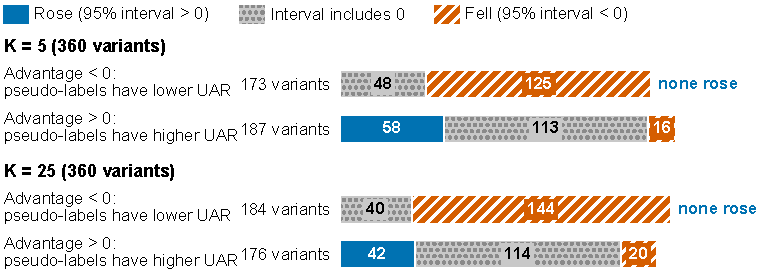
\includegraphics[width=\textwidth]{figures/fig_margin_counts_en.pdf}
\caption{Variants (360 per K; K = 5 and 25) counted by the sign of the advantage and by the 95\% interval of the gain (above zero, including zero, below zero). One variant is one combination of corpus, retrained classifier and pseudo-label provider; the gain is the difference in test UAR. No variant with a negative advantage rose}\label{fig:margincounts}
\end{figure}

Among unimodal classifiers, the one whose K-label baseline had the highest candidate UAR (hereafter the corpus's strongest modality) was visual on AFEW, audio on IEMOCAP, visual on MOSEI and text on MELD at both K = 5 and 25 (on MOSEI, visual and audio differed by only 0.24\pt\ at K = 25: 37.80 vs 37.56). Retraining the classifier of the strongest modality on pseudo-labels from the classifier on the concatenated features of the other two modalities gave negative gains in point estimates for all four corpora and both K (AFEW visual $-$4.40 and $-$3.24, MELD text $-$3.75 and $-$4.21, IEMOCAP audio $-$1.34 and $-$1.02, MOSEI visual $-$3.31 and $-$1.48\pt\ at K = 5 and 25), and six of these eight cases (AFEW, IEMOCAP, MELD) had negative advantages.

\subsubsection{Audio features predicted the text classifier's decisions better than visual features}
On the three corpora other than AFEW, the predictability $D$ of the text classifier's decisions was 19.3 (IEMOCAP), 10.5 (MOSEI) and 17.7 (MELD) points with audio features and 2.0, 0.3 and 3.8 with visual features; the differences (+17.3, +10.2, +13.9) all had intervals above zero. Audio features did not meet the pre-set rule at K = 5 for predicting the visual classifier's decisions better than text features. $D$ may also include agreement from arousal, speaker attributes, utterance duration and recording conditions. Reversing the speech lowered $D$ to 10.5, 3.1 and 10.5 (differences 8.8 [3.0, 14.7], 7.5 [6.3, 8.6] and 7.2 [4.7, 9.8]) (Fig.~\ref{fig:reverse}), but reversed audio still exceeded visual features (by 8.5 [3.8, 13.1], 2.7 [1.3, 4.1] and 6.7 [3.8, 9.6]). Audio's prediction of the text classifier's decisions was therefore not explained by intelligible words alone; the remainder may come from the average spectrum, the pitch distribution, utterance duration, intensity differences within an emotion label or word information left in WavLM features, which this experiment cannot separate.

\begin{figure}[t]
\centering
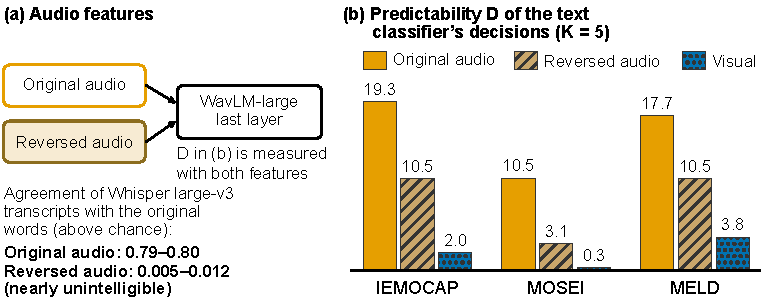
\includegraphics[width=\textwidth]{figures/fig_reverse_en.pdf}
\caption{Predictability $D$ of the text classifier's decisions at K = 5 (UAR points) by original audio, time-reversed audio (words nearly unintelligible) and visual features. The visual value is the reversed-audio $D$ minus the measured difference (reversed audio $-$ visual). AFEW is excluded because its text is a transcript of its own audio}\label{fig:reverse}
\end{figure}

\subsection{Answer to RQ1(b)}
In cross-corpus MER with a few labels per emotion, distillation raised the point estimate of audio UAR above the K-label baseline in all 12 conditions, with intervals above zero in the nine conditions other than IEMOCAP, in the same direction as Albanie et al.\ \cite{albanie2018}, who trained audio classifiers on facial predictions. The 11 methods that do not use pseudo-labels including other modalities were all lower than distillation for audio in point estimates.

Among the 360 post hoc variants per K, the variants whose UAR rose were all ones whose pseudo-labels had higher UAR than the classifier being retrained: advantages and gains ranked together, and no variant with a negative advantage rose. This suggests using pseudo-labels only when they have higher UAR than the classifier to be retrained. One possible explanation of the audio gains is that audio was not the strongest modality on the corpora other than IEMOCAP, and that audio features predicted the text classifier's decisions better than visual features; both come from analyses after the computation and do not establish causes.

Conversely, the classifier of each corpus's strongest modality lost UAR in point estimates in all eight cases when retrained on pseudo-labels from the classifier on the other two modalities. The strongest modality differed across corpora (visual on AFEW and MOSEI, audio on IEMOCAP, text on MELD), and the equal-weight product does not use these differences. Section~\ref{sec:rq2} therefore changes the weights of the three classifiers' predictions per corpus and emotion to raise the UAR of the pseudo-labels.
